
\chapter{Methodology}

To achieve the goal of detecting sugar beet plants, the presented YOLOv5 is used. The exact goal is to develop a preprocessing algorithm which standardizes images of sugar beets for a damage prediction regression task. As described, the images should be standardized in a way that each picture contains one sugar beet plant photographed in a $ 90° $ angle to the ground from above. To train the network on the dataset, a nvidia gpu with 24267 MiB memory was used.

In the following, the given dataset, the training of the network, the evaluation of the models and mobile detection  will be presented.

\section{Dataset}

There are essentially two sources for images of sugar beets and other plants available. One part consists of images taken in sugar beet fields and the other one is Imagenet (\cite{deng2009imagenet}) where a large number of different images with classes is available.

The number of images of sugar beet plants is 10087. This set can be categorized in multiple different types called (1), (2), (3) and (4). The first type is an image with many small sugar beets. The other one is an image with older and bigger plants where the concrete object boundaries are hard to see. One example for each class (1) and (2) can be seen in figure \ref{fig:image_types}.

\begin{figure}[htb!]
	\begin{subfigure}{.6\textwidth}
		\centering
		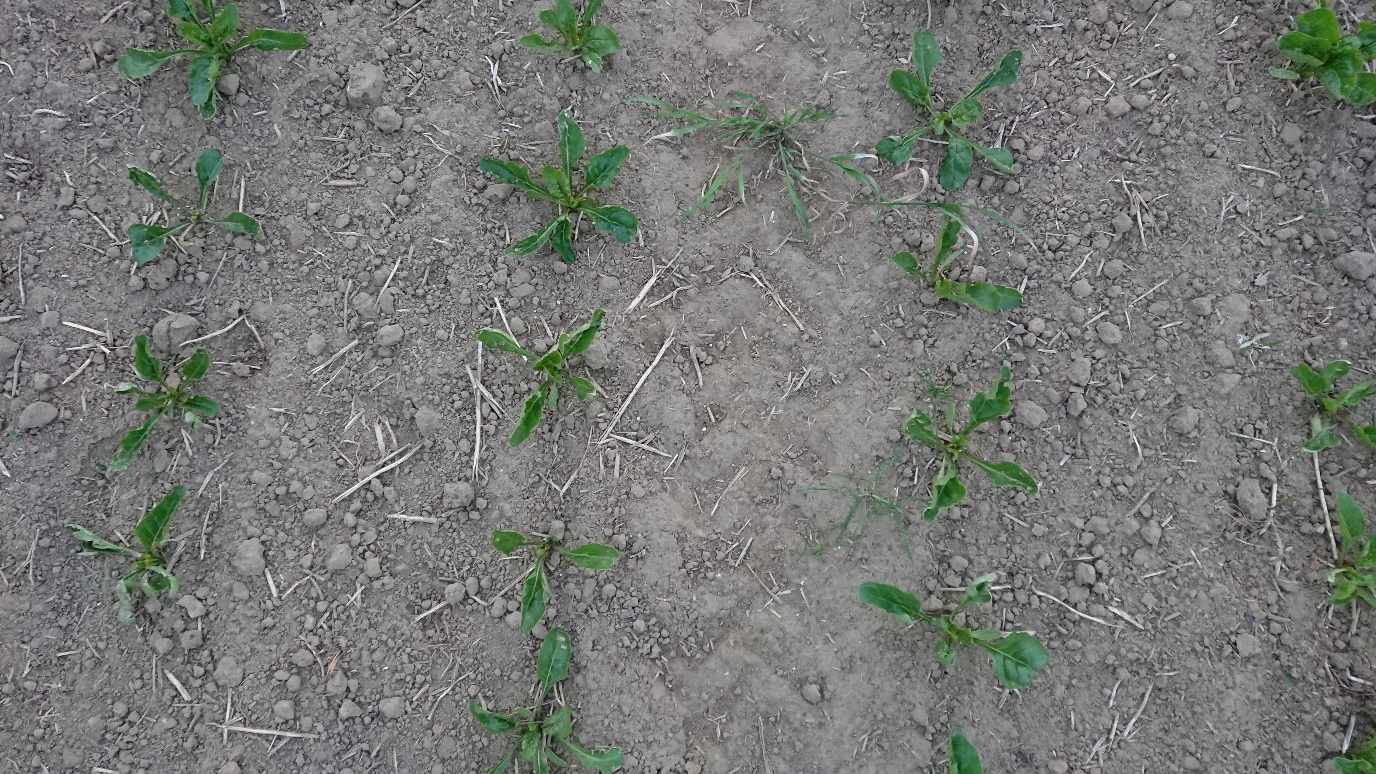
\includegraphics[scale=0.18]{figures/image_type1.JPG}
		\caption{Image type (1). Shows multiple small plants and the boundaries can be seen perfectly.}
		\label{fig:type_1}
	\end{subfigure}%
	\begin{subfigure}{.4\textwidth}
		\centering
		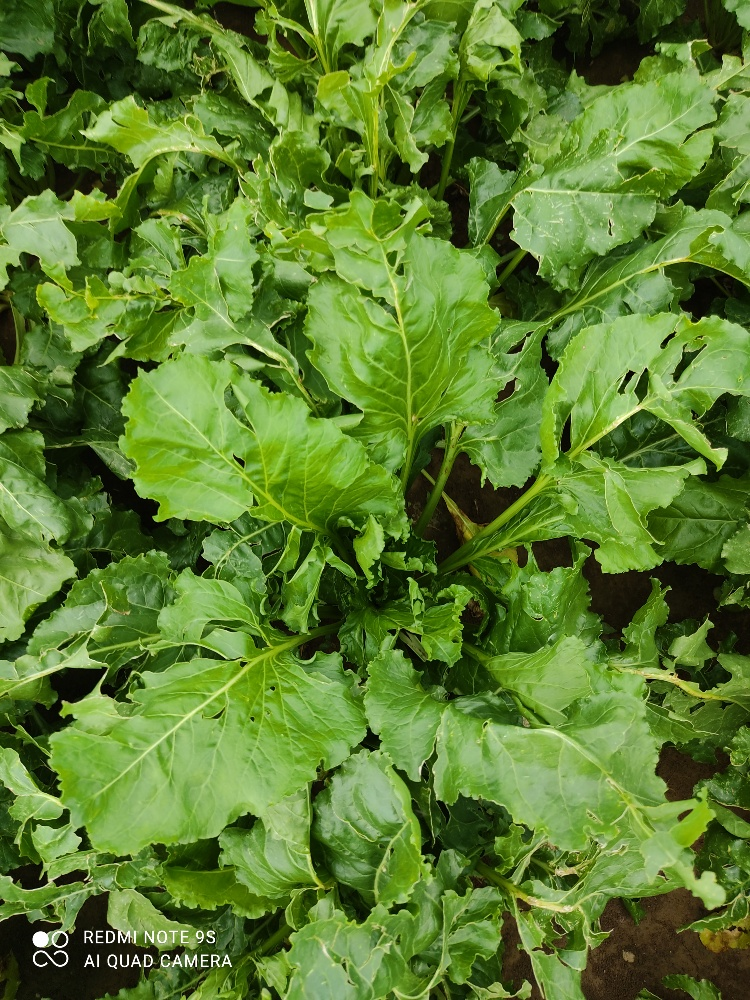
\includegraphics[scale=0.17]{figures/image_type2.jpg}
		\caption{Image type (2). Shows one larger plant, boundaries are overlapping with neighboring plants.}
		\label{fig:type_2}
	\end{subfigure}
	\begin{subfigure}{.6\textwidth}
		\centering
		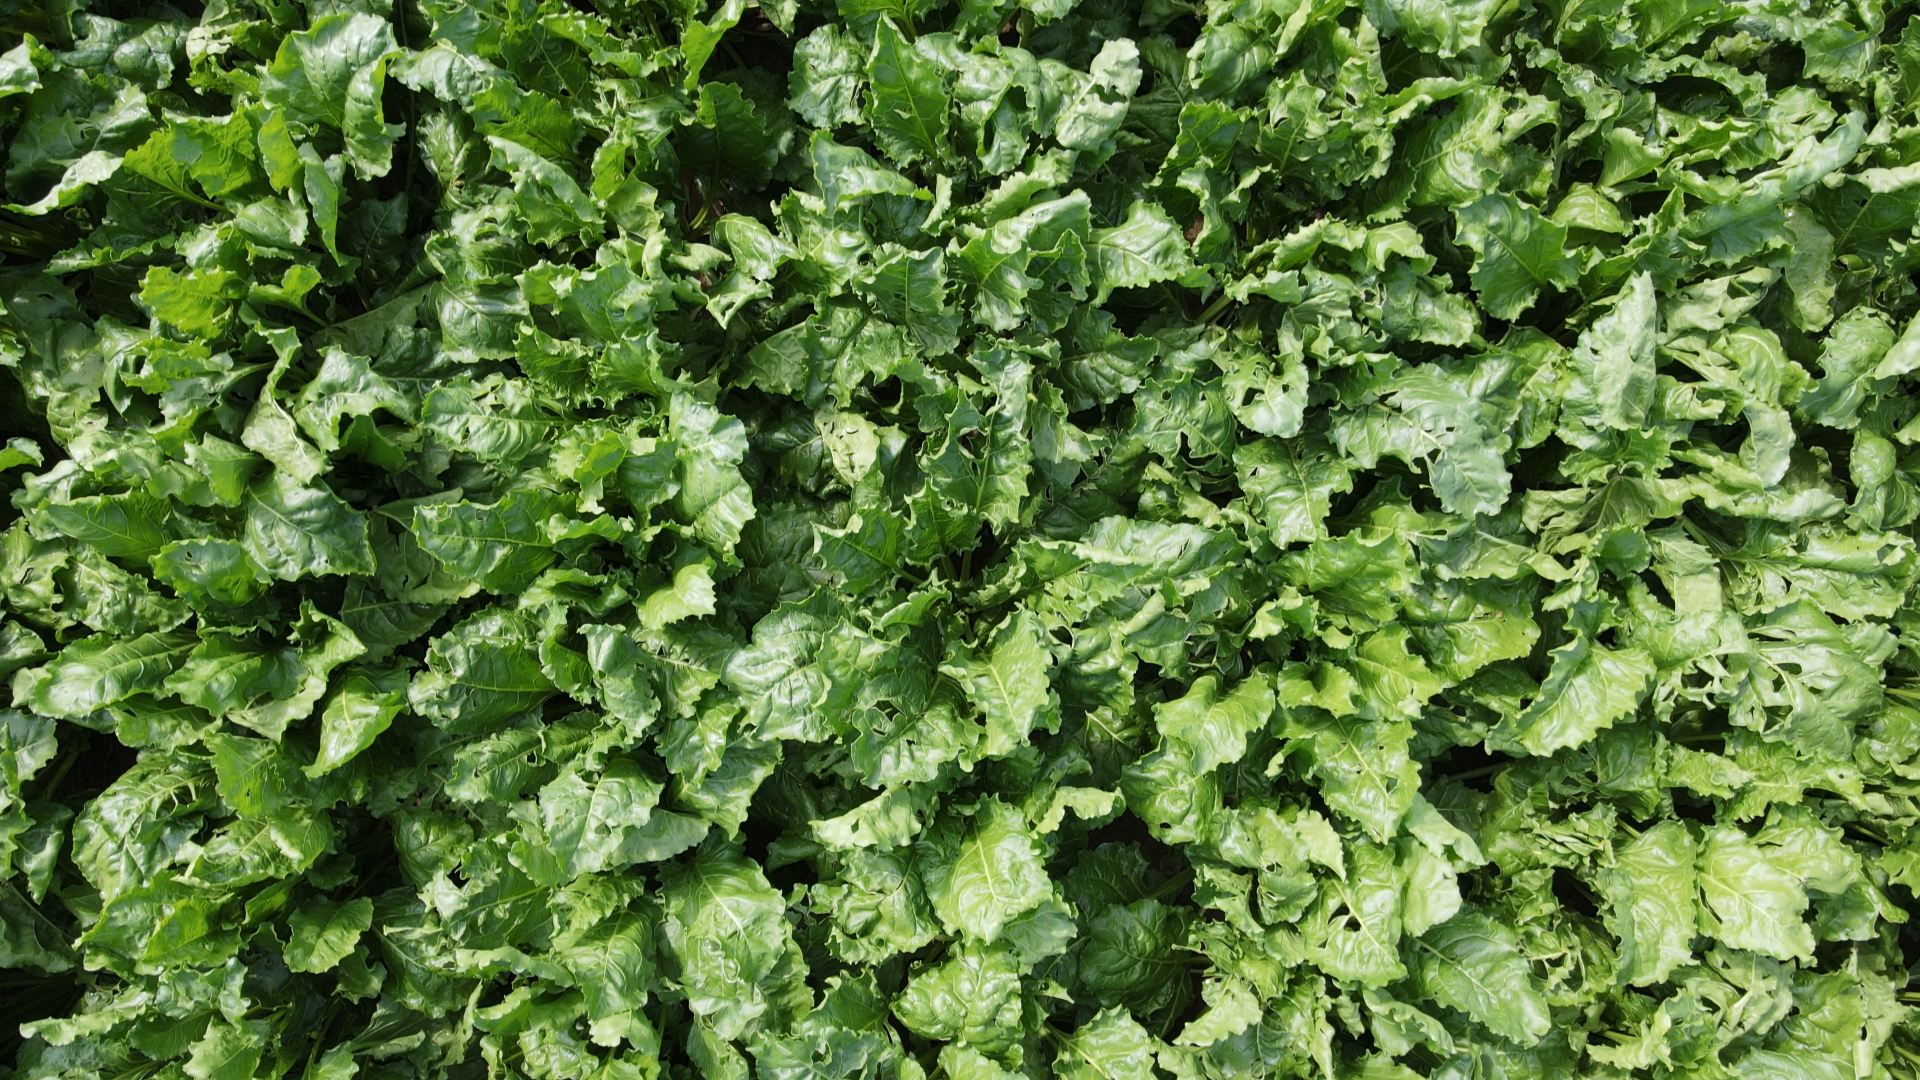
\includegraphics[scale=0.13]{figures/type_4.png}
		\caption{Image type (3). Shows many larger plants. The boundaries of single sugar beets can hardly be seen.}
		\label{fig:type_3}
	\end{subfigure}
	\begin{subfigure}{.4\textwidth}
	\centering
	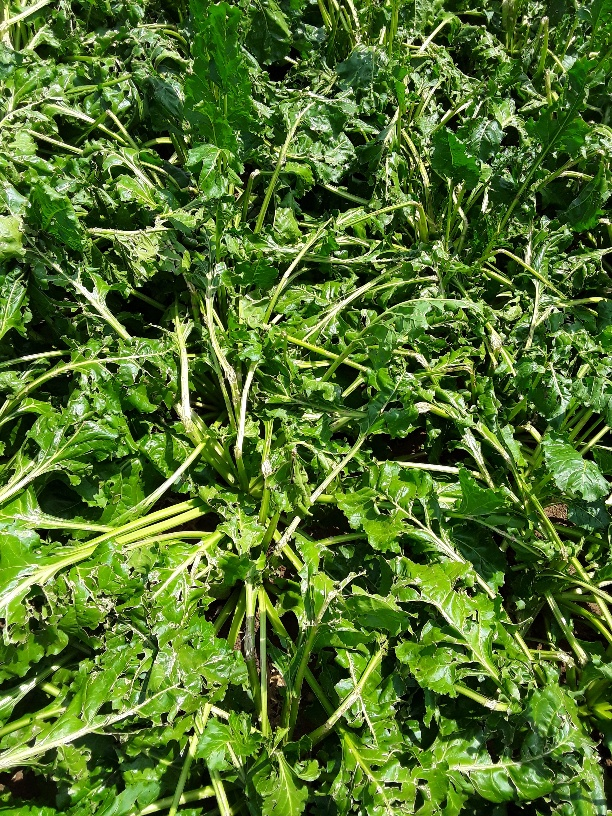
\includegraphics[scale=0.21]{figures/type_3.jpg}
	\caption{Image type (4). Shows plants from a different angle than $ 90° $.}
	\label{fig:type_4}
	\end{subfigure}
	\caption{Example images of types (1), (2), (3) and (4).}
	\label{fig:image_types}
\end{figure}

The first one (\ref{fig:type_1}) is taken from further away and contains multiple smaller plants. The object boundaries can be seen very clearly. This is not the case for the second image type which is depicted in figure \ref{fig:type_2}. It contains bigger plants and the boundaries can not be seen clearly because of the neighboring plants. It is not even easy for the human eye to make find the leafs of a distinct plant. The majority of the whole dataset is of the second type. An example of the third image type can be seen in figure \ref{fig:type_3}. It is a screenshot of a drone video and contains multiple larger plants. Also in this case, the object boundaries can not be seen very clearly because of the overlapping leafs. The last type can be seen in figure \ref{fig:type_4}. This is an example of the images provided by the partner. In general, these pictures are not taken in a standardized way. For example in this case, the angle of the camera is not $ 90° $ and multiple plants can be seen from the side. All in all, figure \ref{fig:bar_chart} shows an overview over the number of images of each type. The row with pictures from Imagenet describes the images taken without any labeling. They do not contain any objects of type sugar beet. Figure \ref{fig:bar_chart} visualizes the distribution. \\

%\begin{table}[h!]
%	\centering
%	\begin{tabular}{|c c c|}
%		\hline
%		Source & Number images & Type \\ % [0.5ex] 
%		\hline\hline
%		TUM & 9461 & (1) \\
%		TUM & 123 & (2) \\
%		Drone screenshots & 244 & (3) \\
%		Partner & 259 & (4) \\
%		Imagenet & 2992 & persons/ other plant\\
%		\hline
%	\end{tabular}
%\end{table}
\begin{figure}
	\centering
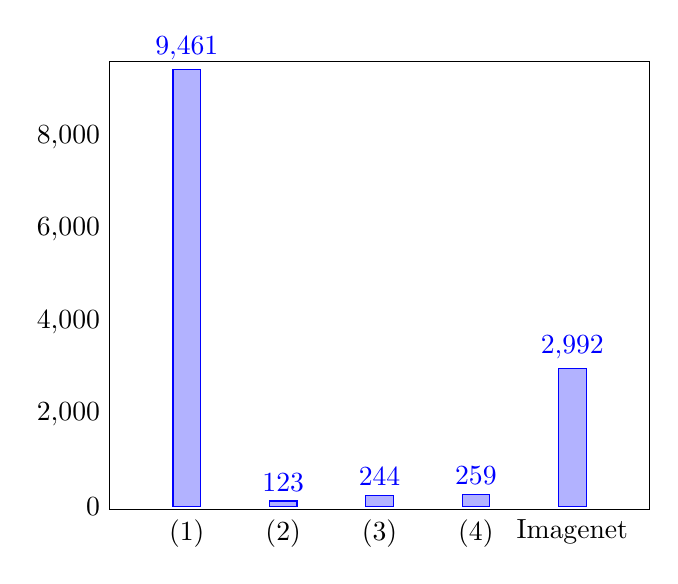
\begin{tikzpicture}
\begin{axis} 	 [
ybar,
tickwidth         = 0pt,
enlarge x limits  = 0.2,
enlarge y limits  = 0.02,
nodes near coords,
symbolic x coords = {(1), (2),
	(3), (4), Imagenet},
]
\addplot coordinates { ((1),9461) ((2),123)
	((3),244) ((4),259) (Imagenet,2992) };
\end{axis}
\end{tikzpicture}
\caption{Overview over the data set with the available images. (1) and (2) are given by TUM. Images of type (3) are screenshots from drone videos and (4) from partner.}
\label{fig:bar_chart}
\end{figure}

The numbers of images for each type are 9461 for the first type and 123 for the second one. They are all provided by TUM. In practice, most images will be of bigger plants because the damage prediction is more important in those cases. 244 images are of type (3) and they are all screenshots from drone videos. Partner provided 259 usable images and they are of type (4). Additionally, Imagenet was used. 2992 images with other plants, flowers and persons were used. These images were not labeled at all. An exact labeling by hands could have been possible but due to time constraints and the fact that only the boundaries of sugar beets have to be detected exactly, this was not done. Possible other solutions would have been to include multiple other classes like concrete plant types or "person" but this is not needed in this application.\\

To train the network, the pictures have to be labeled. For each image file, one text-file has to be made which contains the information of the image. For each object, one line with five numbers has to be added. The first one is the class. The second and third one are the coordinates of the center of the bounding box (x- and y-coordinate). These have to be relative to the width and height of the image. The third and fourth ones are the length in x- and y-direction. They also have to be relative to the image's height width. First experiments showed that the labeling has to be done manually to obtain reasonable results. It could be seen that only labeling the images with multiple small plants and annotating the other ones automatically with \texttt{0 0.5 0.5 1 1} is not sufficient to detect the exact boundaries of bigger plants. Such a labeling exactly means that the center of the bounding box is in the middle and the boundaries are exactly the same as the image boundaries. In most cases, the whole image was detected as a whole sugar beet plant, which was definitely not the goal. The manual labeling was done with the tool labelImg by \cite{labelimg} which provides a graphical user interface to draw the rectangles around the objects. An example of such a labeling of a bigger plant can be seen in figure \ref{fig:labeling}.

\begin{figure}[htb!]
	\centering
	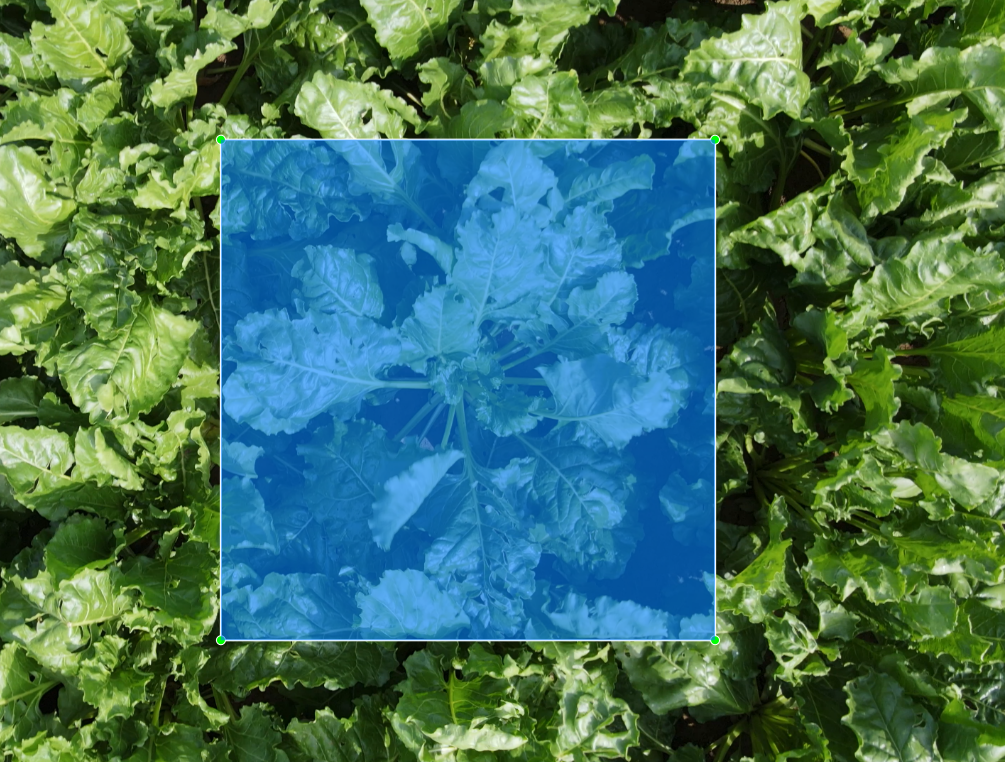
\includegraphics[scale=0.2]{figures/labeling.png}
	\caption{Labeling images with labelImg which provides a graphical user interface to draw bounding boxes into the pictures.}
	\label{fig:labeling}
\end{figure}

As you can see in this figure, the plant in the center of the image is labeled as sugar beet. The rectangle of the object has to be as exact as possible to obtain best results in predictions. Although especially in the case of big plants, this is not always easy because neighboring sugar beets are overlapping and the plant boundaries can not even be seen very clearly with the human eye. Nevertheless, all available images were labeled manually to get best possible results. An overview of the complete data set can be seen in figure \ref{fig:bar_chart}.\\

All in all, the most available images contain about one larger plant from above which can also be seen in figure \ref{fig:bar_chart}. The biggest variety of image types can be seen from the Partner. These were taken in very different angles and contain various damages ranging from nearly no to high destruction. The drone screenshots are similar to the TUM data set but are taken from a bit more far above. The drones captured most of the time more than one large plant at a time resulting in overlapping sugar beets again. This overview in the figure \ref{fig:bar_chart} shows that much data was gathered and labeled. Compared to the use case where the plants should be detected, the available data is very suitable for the application as it has many different cases ranging from many plants on one images to only containing one sugar beet. Also the damage classes are distributed meaning that images with very different degree of damage are available.

\section{Training}
For the training of the YOLOv5 model, different parameters and other settings have to be specified. One first thing is the decision between different model sizes. As described in the description of YOLOv5, there are different possibilities. The ones we are concentrating on are the small, medium, and large one. For each of them, a pretrained model on the COCO data set by \cite{COCO} with 300 epochs and default settings are available (\cite{yolov5}). This data set contains 328 thousand images with 2.5 million instances of 91 object classes. Alternatively, the raw model without pretraining can be used. In a configuration file, many different hyperparameters can be adjusted such as box, class and obj loss gain. Also the IoU (intersection over union) training threshold can be set. This value determines the fraction of the area of the intersection of two bounding boxes over the union of them. The highest achievable value is 1 which means that the predicted box is exactly the same as the labeled box. Many other parameters for image augmentation are also available. One example therefore is hue, saturation, and value which are then just changed in the image. Also degrees of rotation, translation, scaling, shearing and the perspective can be adjusted. More complex ones are the probability of flipping the image upside down or left-right, respectively. Additionally, mosaic can be chosen. This means that many different images with their labels are concatenated to form a larger image. Also the probability for mixup and copy paste can be chosen independently. Examples for the last three augmentations can be seen in figure \ref{fig:augmentation}.\\


\begin{figure}[htbp!]
	\centering
	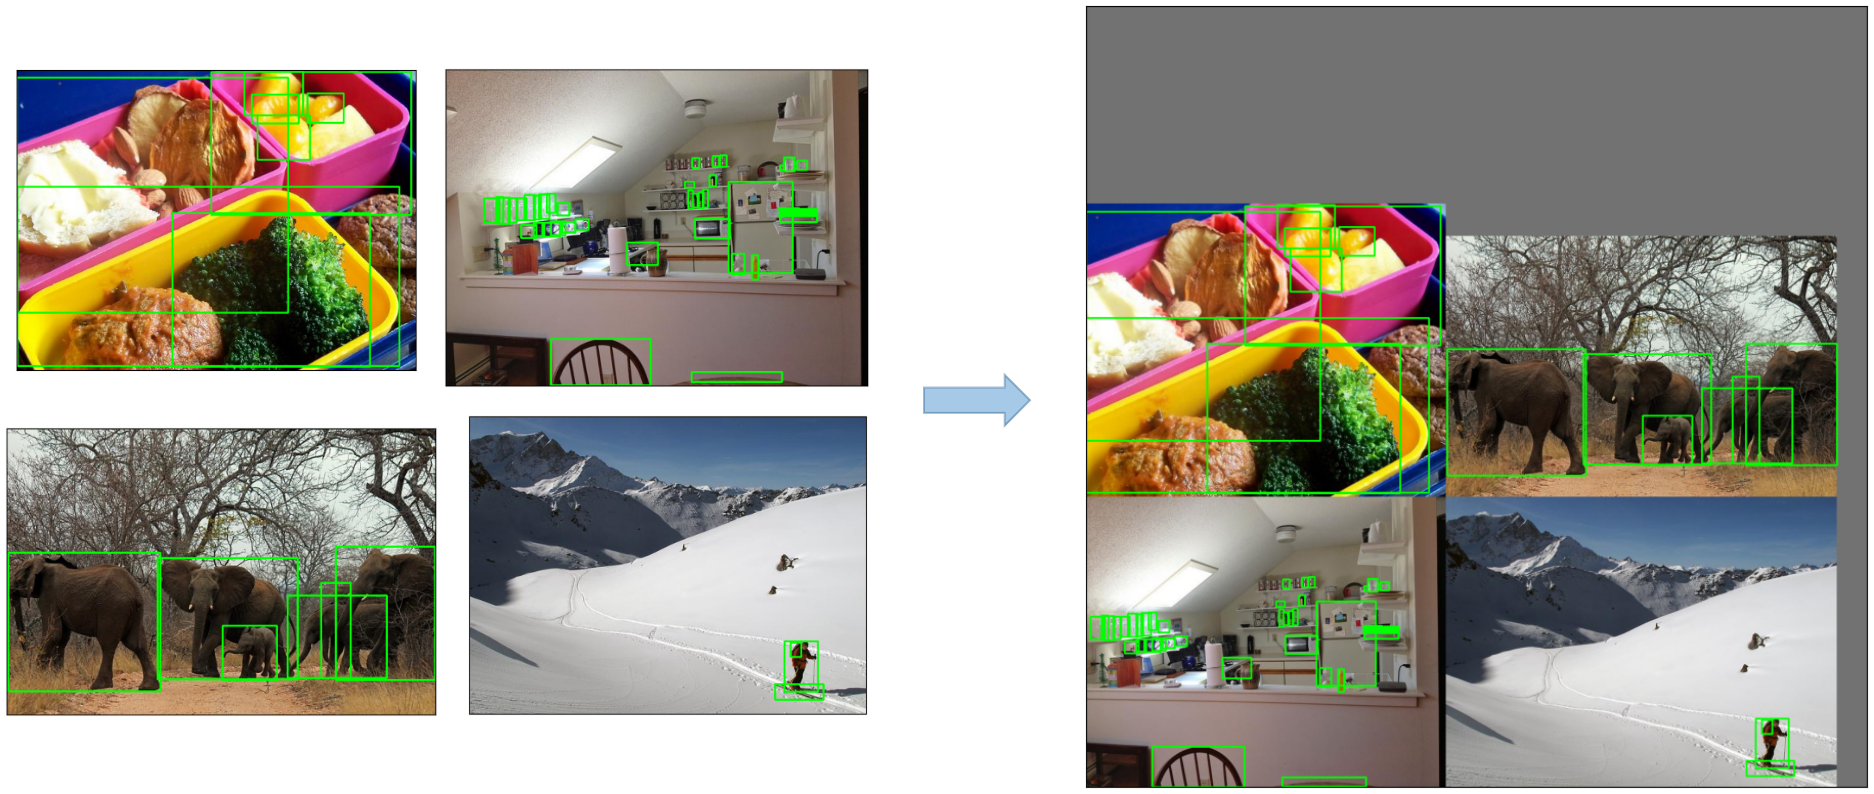
\includegraphics[scale=0.18]{figures/mosaic.png}
	\hspace{40pt}
	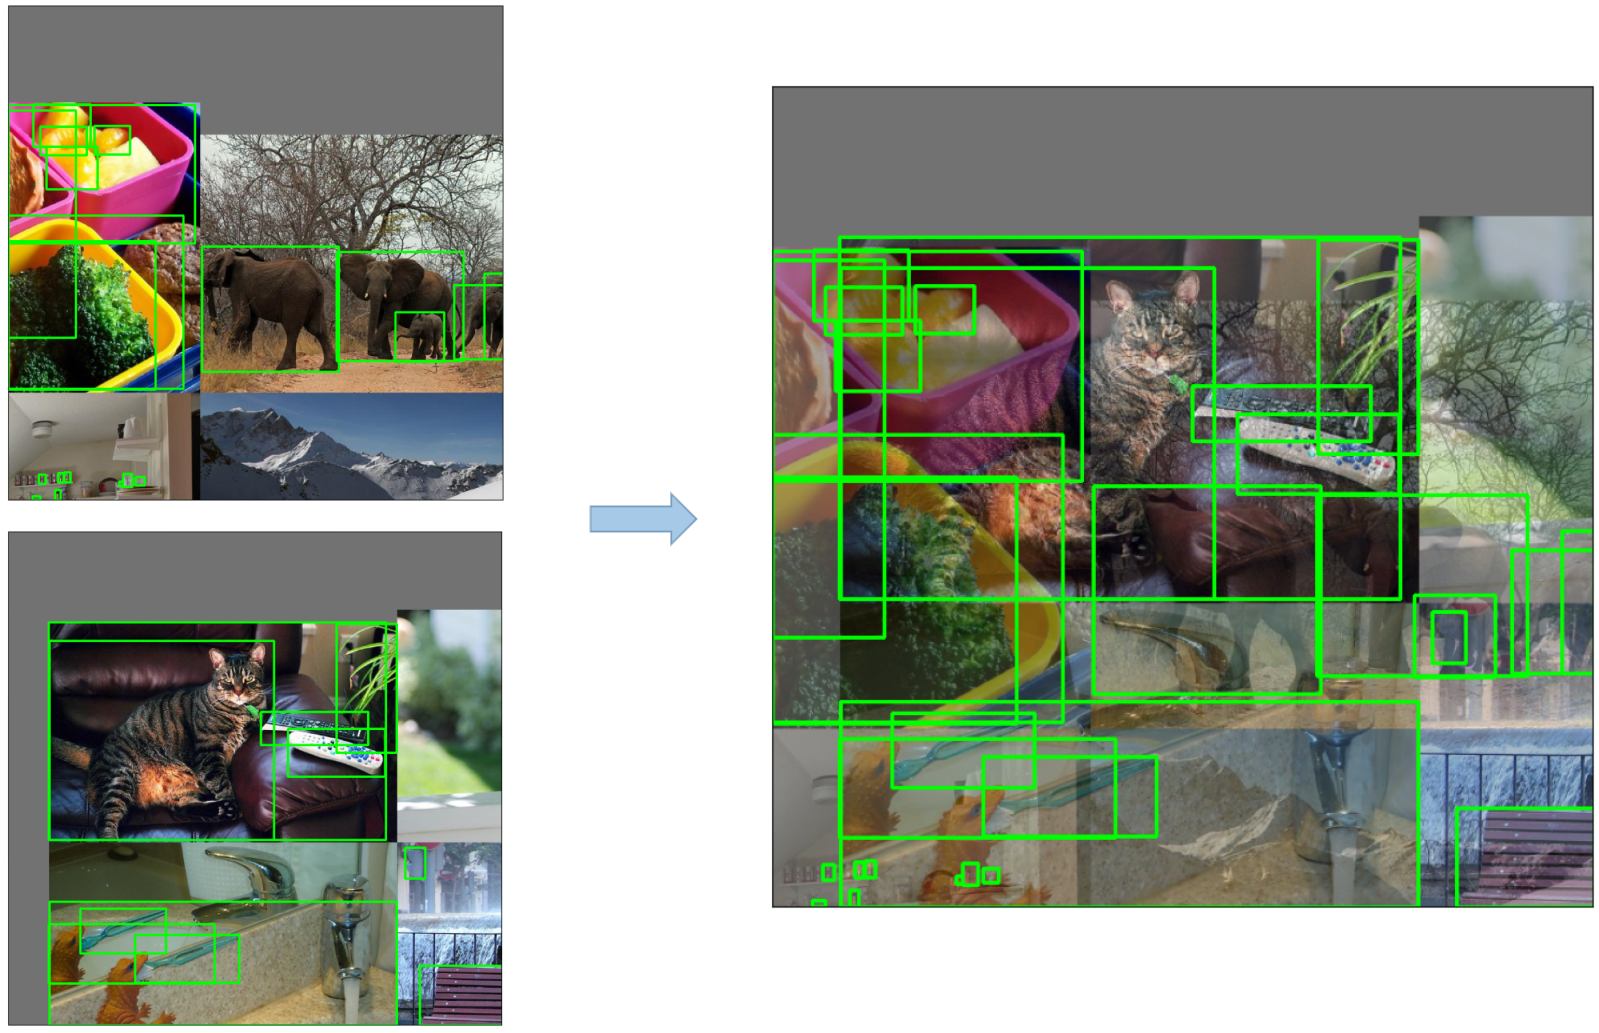
\includegraphics[scale=0.18]{figures/mixup.png}
	\hspace{40pt}
	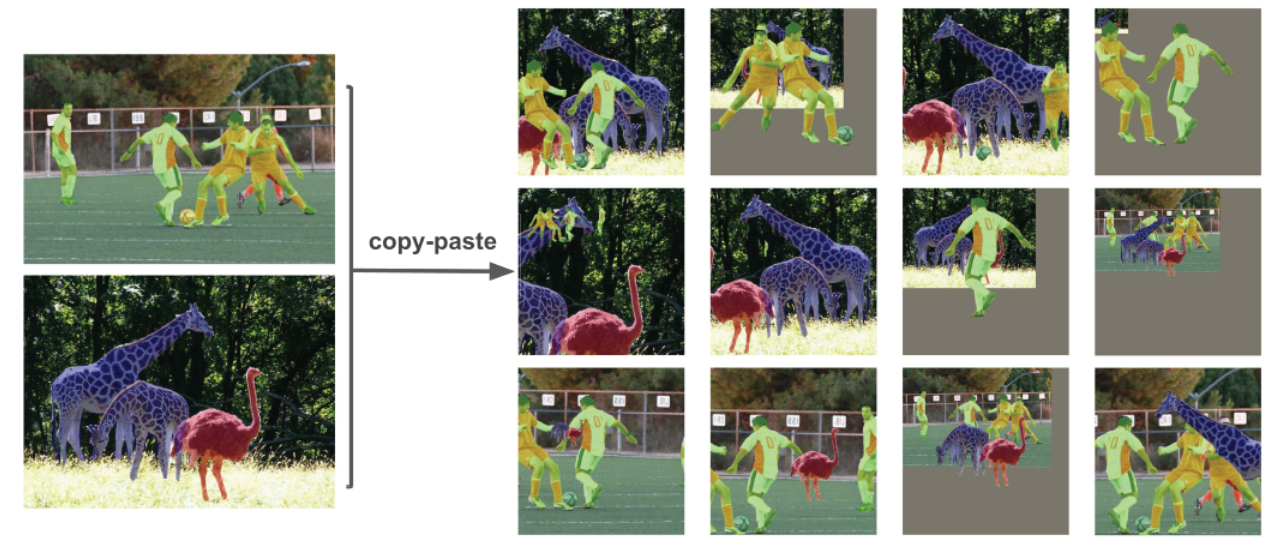
\includegraphics[scale=0.27]{figures/copy-paste.png}
	\caption{Data augmentation types. These techniques can be used to combine different images as new input for training. The first row shows mosaic which just concatenates them. Middle row is mixup laying several images behind each other. Last row is copy-paste which duplicates different objects into other pictures. Taken from \cite{yolov5}}
	\label{fig:augmentation}
\end{figure}

Depicted in the top row, mosaic just puts different labeled images together in a random way to form one larger training image. In the middle row, mixup augmentation is depicted. This one is more complex because it copies multiple labeled image overlapping into a larger one. The bottom row depicts the copy paste augmentation which copies single instances of classes to other labeled training images. All in all, these different augmentation strategies help to improve the model's robustness because the variety of input images is increased. 

Further settings that have to be made to train the models are defining the train, validation, and testing split. Additionally, the number of epochs can be defined. As optimizer, SGD (stochastic gradient descent), Adam, and AdamW can be chosen. The concrete training scenarios and their settings will be described in the results. 

\section{Inference and Evaluation}
For the detection of objects, multiple different inputs are possible. Either the images of whole folders, single pictures, or the live stream of the webcam can be processed. In each way, the image is directly labeled with the bounding box of the detected class. Additionally, it is possible to write the result to a text file in the same format as the label for the training images. \\

To evaluate the model's accuracies, the test set is used. Metrics like the precision and the recall can be directly measured with the framework by \cite{yolov5}. Precision and Recall are calculated with  
\begin{equation}
P = \frac{T_p}{T_p + F_p},\textrm{ } R = \frac{T_p}{T_p + F_n} 
\end{equation} 
with $ T_p $ true positive, $ F_p $ false positive, and $ F_n $ false negative predictions.\\

For the three model sizes, different inference times can be observed. For the small one, the prediction takes about 100ms, the medium one takes about 224ms and the slowest is the large one with about 450ms. All times are taken on a normal CPU. \\

For a live application detecting the objects, the large model is definitely too slow. It takes too much time to detect objects and the live stream updates not fast enough. Even with the medium model, the window is not fluent. Using the small model, a live application detecting the sugar beets can be done. The inference times are not too high to still give a fluent live image. \\

These inference times leave room for two versions. The first one is just processing the image taken from the field on the server where also the regression model is implemented. The second one is using the model directly in the app so that the user can also see and maybe interact with the bounding boxes of the predicted sugar beets. \\

As a metric for evaluating how the network performed, the area under curve (AUC) of the P-R-curve is used. This measures the mean average precision of the model which is in our case (only one class sugar beet) the average precision. For other metrics that can be used in object detection, refer to the survey by \cite{metrics_survey}.

\section{Mobile Detection}
For the detection directly in the app, Pytorch mobile \cite{pytorch_mobile} can be used. For an overview of machine learning in mobile applications, refer to \cite{survey_machine_learning_mobile}. \\

For the application, the pt file of the model can be used to detect objects directly in the application. This would have the advantage that the user can directly see whether a sugar beet is detected and adjust his angle or distance to the plant. Additionally possible would be to let the user adjust the bounding box if he thinks that the prediction is not precise enough. 


